\documentclass[twoside]{layout/siccs-thesis}

%% for equations a  nice parameter description
\newenvironment{conditions}
  {\par\vspace{\abovedisplayskip}\noindent\begin{tabular}{>{$}l<{$} @{${}={}$} l}}
  {\end{tabular}\par\vspace{\belowdisplayskip}}


%%  spacing before and after equations to the text
\setlength{\abovedisplayskip}{8pt}
\setlength{\belowdisplayskip}{8pt}

%% top margin headheght
%\setlength{\headheight}{13.59999pt}
\setlength{\headheight}{14pt}


%% Set up the bibliography
% styles   https://de.overleaf.com/learn/latex/Biblatex_citation_styles
% here is the used bibliography package
%\usepackage[style=authoryear,sorting=nyt,maxcitenames=3]{biblatex}
\usepackage{biblatex}
\addbibresource{references.bib}

% for spacing between references in the bibliography
\setlength\bibitemsep{1.5\itemsep}

% for the commas between author and year
\DeclareDelimFormat{nameyeardelim}{\addcomma\space}

%% Additional packages and commands

%settings for the SI units
\sisetup{locale = DE,
output-decimal-marker={.}, % because  in german is switched to {,}
separate-uncertainty=true,  
multi-part-units=single,
range-units = single ,  
list-units = single,  
per-mode=reciprocal,
group-minimum-digits = 4,
number-unit-product = \hspace{0.16667em plus 0.08334em}}


%% here individual units are defined 
\DeclareSIUnit\equivalents{eq}
\DeclareSIUnit\water{kgw}
\DeclareSIUnit\year{yr}
\DeclareSIUnit\dollar{\$}

\setlist{itemsep=-2pt} % Reducing white space in lists slightly
\renewcommand{\deg}{\si{\degree}\xspace} % Use \deg easily, everywhere


%%%%%%%%%%%%%%%%%%%%%%%%%%%%%
%%%%% Begin of document %%%%%
%%%%%%%%%%%%%%%%%%%%%%%%%%%%%

\begin{document}

%% Roman page numbering
\frontmatter

%% Defining the main parameters
\title{Title of the thesis}
\subtitle{Master Thesis}
\author{Your Name}
%\subject{AB1234: Optional Course Name}
\affiliation{University of Hamburg}

\definecolor{title}{HTML}{4884d6} % Color for title

%this only made for the first commit to check if everthing is sinc
% title page
%----------------------------------------------------------------------------------------
%	TITLE PAGE
%----------------------------------------------------------------------------------------

\begin{titlepage} % Suppresses headers and footers on the title page
\frontmatter

%\vspace*{-4cm}
%\hspace*{-1.5cm}
%\includegraphics[height=3cm]{Figures/general/up-uhh-logo.png}
%\hfill
%\includegraphics[height=3cm]{Figures/general/DESY_logo_4C.png}

\vspace{2cm}
    \centering

	%\vspace{2.\baselineskip} % Whitespace above the title
	%\vspace{-2cm}
%	\noindent\makebox[\linewidth]{\rule{1.05\textwidth}{1.5pt}} \\
	%\rule{\textwidth}{1.5pt}\\
	\vspace{0.4cm}
    \parbox[t]{0.96\textwidth}{\rmfamily \setlength\parfillskip{0pt} \def\baselinestretch{1.1}\centering\Huge \bfseries My GitHub title}\\
	\vspace{0.4cm}
%	\noindent\makebox[\linewidth]{\rule{1.05\textwidth}{1.5pt}} \\
    %\rule{\textwidth}{1.5pt}\\
    \vspace{2 cm} % Whitespace below the title
	
	
    \parbox[p]{0.95\textwidth}{\def\baselinestretch{1.4}\centering\scshape\textbf{\LARGE Dissertation} \\ {\large zur Erlangung des Doktorgrades an der Fakult{\"a}t\\ f{\"u}r Mathematik, Informatik und Naturwissenschaften \\ Fachbereich Physik \\ der Universit{\"a}t Hamburg} }
    
    \vspace{2 cm} % Whitespace after this block

    \parbox[b]{0.93\textwidth}{\def\baselinestretch{1.3}\centering\upshape \large vorgelegt von \\ {\LARGE\scshape  Andrei Trebushinin} \\ %aus \\ {\scshape \bfseries XXXXXX}
    }
    
    \vspace{2 cm} % Whitespace after this block
    
    \parbox[b]{0.93\textwidth}{\def\baselinestretch{1.3}\centering \large\scshape Hamburg\\\scshape 2023}

\end{titlepage}

%----------------------------------------------------------------------------------------
%----------------------------------------------------------------------------------------
 
 
\vfill\vspace{-2cm}\par
\thispagestyle{empty}
%\cleardoublepage

\thispagestyle{empty}
\section*{Eidesstattliche Erkl\"arung / Declaration on oath}
\vspace{1cm}
\begin{center}
    
\parbox[b]{0.85\textwidth}{
  
Ich erkl\"are hiermit an Eides statt, dass ich diese Dissertation selbst verfasst und keine anderen als die angegebenen Hilfsmittel oder Quellen benutzt habe.\\

I hereby declare in lieu of oath that I have written this dissertation myself and that I have not used any auxiliary materials or sources other than those indicated.\\\\
\vspace{1cm}

\hspace{0.2cm} Hamburg, \today \hfill 
\vspace{0.5cm}

\hfill Unterschrift des Doktoranden \hspace{1.0cm} 
}

\end{center}
\vfill

\newpage
\thispagestyle{empty}
\cleardoublepage

\newpage
\thispagestyle{empty}
\parbox[b]{\textwidth}{
\renewcommand{\arraystretch}{2.0}
\begin{tabular*}{\linewidth}{p{0.6\linewidth}p{0.4\linewidth}}
 
% (alle Angaben vorl\"aufig) & \\ \\
 
 Gutachter/innen der Dissertation:
  & Dr. 1\\
  & Prof. Dr. 2\\ 
  \\
  
 Zusammensetzung der Pr{\"u}fungskommission: 
  & Prof. Dr. 1 \\
  & Prof. Dr. 2 \\
  & Dr. 3 \\
  & Jun.-Prof. 4\\
  & Dr. 5\\
  
 Vorsitzende/r der Pr{\"u}fungskommission: & Prof. Dr. 1\\
 \\
 
 Datum der Disputation: & 00.00.2024 \\
 \\
 
 Vorsitzender des Fach-Promotionsausschusses PHYSIK: & 1 \\
%Vorsitzende des Promotionsausschusses: & Prof. Dr. Jan Louis \\
 \\

 Leiter des Fachbereichs PHYSIK: & 1 \\
%Leiter des Fachbereichs Physik: & Prof. Dr. Peter Hauschildt \\
 \\

 Dekan der Fakult{\"a}t MIN: & 1 \\
%Dekan der Fakult\"ar f\"ur Mathematik, & \\
%Informatik und Naturwissenschaften:  & Prof. Dr. Heinrich Graener \\
% 
 \end{tabular*}
 \\ \\ 
 }

\clearpage


% abstract
%\chapter*{Abstract}
\addcontentsline{toc}{chapter}{Summary}

% Abstracts are usually around 100–300 words
\noindent\lipsum[2-4]
\thispagestyle{empty}
\vspace{-3cm}
\section*{\centering Zusammenfassung}

your abstract in German
\noindent

%$\noindent\lipsum[2-4]

% \thispagestyle{empty}
% \mbox{}

\newpage

\thispagestyle{empty}
\vspace{-3cm}
\section*{\centering Abstract}
your abstract in English
\noindent
% \thispagestyle{empty}
% \mbox{}


\newpage

\tableofcontents

\newpage\null\thispagestyle{empty}\newpage
% \listoffigures
% \listoftables
\newpage
%\listoffigures
%\listoftables
%\chapter*{Nomenclature}
\addcontentsline{toc}{chapter}{Nomenclature}


\section*{Abbreviations}

\begin{longtable}{p{2.5cm}p{8cm}}
    \toprule
    Abbreviation & Definition \\
    \midrule\endhead % Abbreviations added alphabetically here:
    USA & United States of America\\
    EU & European Union \\
      \bottomrule
\end{longtable}

\section*{Variable Names}

\begin{longtable}{p{2.5cm}p{8cm}p{2.5cm}}
    \toprule
    Symbol & Definition & Unit \\
    \midrule\endhead % Latin symbols added alphabetically here:
    $\alpha$ & greek alpha & [\si{\newton}] \\
    \midrule
    $\beta$  & greek beta  & [\si{\joule}]   \\
    \bottomrule
\end{longtable}

%% Arabic page numbering
\mainmatter
\pagestyle{fancy}

\setcounter{page}{9}
\chapter{Introduction}


\label{chapter:introduction}

\noindent\lipsum[4-10]



\chapter{Theory}
\label{chapter:theory}


\noindent\lipsum[20-25]

\section{Example Figure}
Make sure to include pdf format (or any vector graphics format) figures in your thesis whenever possible. You will be thankful for it when printing the document. 
\begin{figure}[H]
    %% trim=left bottom right top,
    \centering
   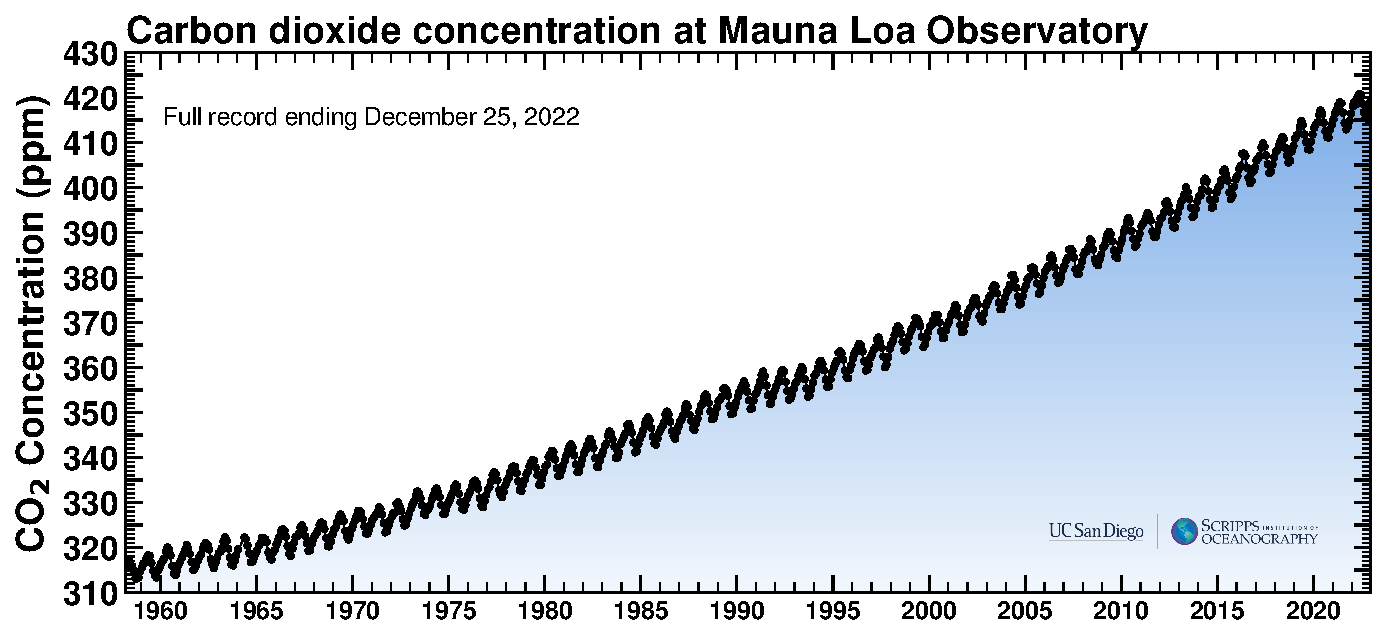
\includegraphics[width=1.0\textwidth,keepaspectratio,trim=0 0 0 0, clip]{figures/mlo_full_record.pdf}
    \caption{ Mauna Loa observatory \ch{CO2} measurement \parencite{keeling-curve} }
    \label{fig:scatter_plot_sand}
\end{figure}


\section{Example chemical reaction}
Carbonic acid deprotonation:
\begin{equation}
    \ch{CO2 + H2O ->[] HCO3^- + H^+}.
\end{equation}

\section{Example of the equation with self-defined conditions environment }
The relative permittivity $\epsilon_{r}$ is defined as: 
\begin{equation}
    \label{eqn:relative_permittivity}
    {\displaystyle \varepsilon _{\mathrm {r} }={\frac {\varepsilon }{\varepsilon _{0}}}}
\end{equation}
\begin{conditions}
    \epsilon & permittivity of the material \\
    \epsilon_0 & vacuum permittivity.\\
\end{conditions}

\section{Example of different citations}
Overall \textcite{arrhenius1896xxxi} calculated that cutting CO2 in half would suffice to produce an ice age. He further calculated that a doubling of atmospheric CO2 would give a total warming of 5–6 degrees Celsius.

\noindent
Overall, Arrhenius calculated that cutting CO2 in half would suffice to produce an ice age. He further calculated that a doubling of atmospheric CO2 would give a total warming of 5–6 degrees Celsius (\cite{arrhenius1896xxxi}).

\noindent
Overall, Arrhenius calculated that cutting CO2 in half would suffice to produce an ice age. He further calculated that a doubling of atmospheric CO2 would give a total warming of 5–6 degrees Celsius \parencite{arrhenius1896xxxi}.

\section{Example list}
\begin{itemize}
    \item first
    \item second
    \item third
    \item fourth
    \item fifth
    \item sixth
    \item seventh
\end{itemize}

\section{Example table}

\begin{table}[H]
\centering
\begin{tabular}{|l|l|}
\hline
\rowcolor{gray!50}
Country (or dependency) & Population (2020) \\ \hline
China                  & 1,439,323,776       \\ \hline
India                  & 1,380,004,385        \\ \hline
USA                    & 331,002,651           \\ \hline
Indonesia              & 273,523,615            \\ \hline
Pakistan               & 220,892,340             \\ \hline
Brazil                 & 212,559,417              \\ \hline
Nigeria                & 206,139,589               \\ \hline
\end{tabular}
\caption{example caption }
\label{tbl:example_table}
\end{table}

\section{Example of siunitx package}
The siunitx package is amazing for controlling all numbers and units of the document globally. You can set everything globally for the document and don't need to change every single number for formatting changes.\\
At the beginning of the document, the settings are made.

%% settings for the SI units from main.tex
% \sisetup{locale = DE,
% output-decimal-marker={.}, % because  in german is switched to {,}
% separate-uncertainty=true,  
% multi-part-units=single,
% range-units = single ,  
% list-units = single,  
% per-mode=reciprocal,
% group-minimum-digits = 4,
% number-unit-product = \hspace{0.16667em plus 0.08334em}}



\begin{itemize}
    \item range of numbers + unit:  \SIrange{3}{10}{\cubic\kilo\meter \per \second}
    \item number + unit : \SI{3}{\cubic\kilo\meter \per \second}
    \item just unit   : \si{\cubic\kilo\meter \per \second}
    \item number + uncertainty + unit \SI{3 \pm 0.1}{\cubic\kilo\meter \per \second}
\end{itemize}

\section{Example colors}
Example of how to use colors in the text.
\begin{enumerate}
\color{blue}
    \item Blue
    \item More blue
    \item {\color{red} And red!}
    \item \begingroup\color{green} lol   \endgroup
    \item {\color{yellow} And yellow!}
\end{enumerate}




%\input{content/chapter-2}
%\input{content/chapter-3}

\chapter{Methods}
\label{chapter:methods}

\noindent\lipsum[10-15]


%\input{mainmatter/chapter-4} % Create file to add

\chapter{Results}
\label{chapter:results}
\noindent\lipsum[15-20]


\chapter{Discussion}
\label{chapter:discussion}


\chapter{Conclusion}
\label{chapter:conclusion}



\newpage
\setcounter{secnumdepth}{-1}
\section*{Acknowledgement} % * title not in table of contents

% some example sentences you could use for the acknowledgement
First, I like to thank my first supervisor .... , for .... . Also, I want to thank my second supervisor .... for .... .\\

\noindent
Thanks to ..... for all the insights into .... . Thanks to .... for all the intense but fruitful scientific debate about .... . Thanks to ... , who always had an open door for ..... . \\

\noindent
Also, I would like to thank the .... . \newline

\noindent
And last but not least, thanks to .... , who helped ..... . As well as .... for the help with .... . 

%% Prevent urls running into margins in bibliography
\setcounter{biburlnumpenalty}{7000}
\setcounter{biburllcpenalty}{7000}
\setcounter{biburlucpenalty}{7000}



%%  Add the bibliography
%\printbibliography[heading=bibintoc,title=References]
\printbibliography[heading=bibintoc,title=References]

% Letters for chapters
\appendix

\newpage
\setcounter{secnumdepth}{-1}

%\chapter*{Eidesstattliche Versicherung}

Hiermit versichere ich an Eides statt, dass ich die vorliegende Arbeit im Studiengang ......... selbstständig verfasst und keine anderen als die angegebenen Hilfsmittel – insbesondere keine im Quellenverzeichnis nicht benannten Internet-Quellen – benutzt habe. Alle Stellen, die wörtlich oder sinngemäß aus Veröffentlichungen entnommen wurden, sind als solche kenntlich gemacht. Ich versichere weiterhin, dass ich die Arbeit vorher nicht in einem anderen Prüfungsverfahren eingereicht habe und die eingereichte schriftliche Fassung der auf dem elektronischen Speichermedium entspricht.\newline

\noindent
Einer Veröffentlichung der vorliegenden Arbeit in der zuständigen Fachbibliothek des Fachbereichs stimme ich zu.\newline


\vspace{25mm}

%  The aligning options are m for middle, p for top and b for bottom. 
\noindent
\begin{tabular}{@{}p{2.5cm}p{3cm}p{2cm}p{7cm}}
Hamburg, den  & \hrulefill & Unterschrift: & \hrulefill \\
\end{tabular}


  



\begin{comment}
    Bei der Abgabe der Abschlussarbeit ist eine Versicherung an Eides statt (lt. § 59 Abs. 3 HmbHG) abzugeben:

„Hiermit versichere ich an Eides statt, dass ich die vorliegende Arbeit im Studiengang ...*) selbstständig verfasst und keine anderen als die angegebenen Hilfsmittel – insbesondere keine im Quellenverzeichnis nicht benannten Internet-Quellen – benutzt habe. Alle Stellen, die wörtlich oder sinngemäß aus Veröffentlichungen entnommen wurden, sind als solche kenntlich gemacht. Ich versichere weiterhin, dass ich die Arbeit vorher nicht in einem anderen Prüfungsverfahren eingereicht habe und die eingereichte schriftliche Fassung der auf dem elektronischen Speichermedium entspricht.“             *) bitte Ihren Studiengang und Abschluss eintragen

Die Angabe zur Veröffentlichung in der Fachbibliothek können Sie direkt in die Versicherung mit einbeziehen:

"Einer Veröffentlichung der vorliegenden Arbeit in der zuständigen Fachbibliothek des Fachbereichs stimme ich zu/stimme ich nicht zu."

Bitte drucken Sie diese Versicherung in jedem Exemplar am Ende ab und unterschreiben Sie diese mit der Angabe von Ort und Datum.
\end{comment}





%\input{appendix/appendix-a}





\end{document}